\subsection{Distance to key residues}

\begin{figure}[!ht]
\centering
  \begin{subfigure}{.45\textwidth}
     \centering
     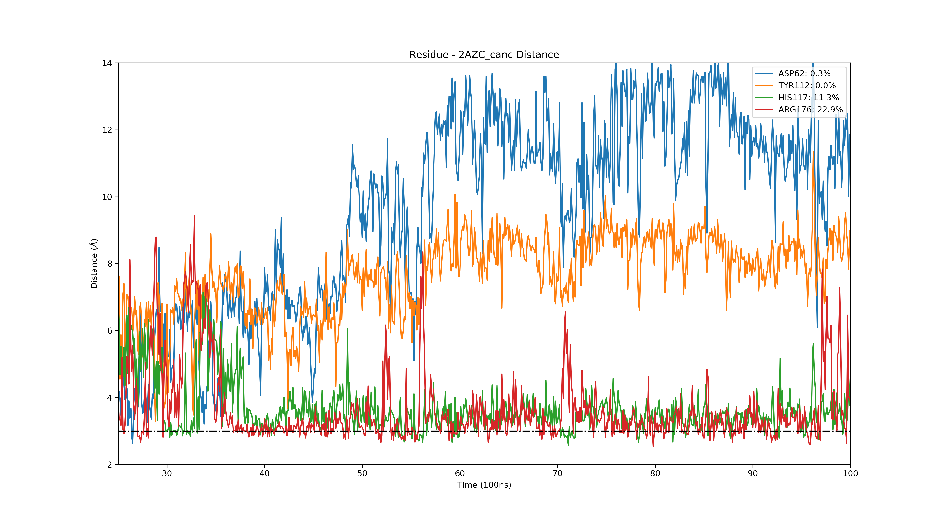
\includegraphics[width=.95\linewidth]{chapter4/2AZC_canc/2AZC_canc-dist_0.pdf}
  \end{subfigure}
  \begin{subfigure}{.45\textwidth}
     \centering
     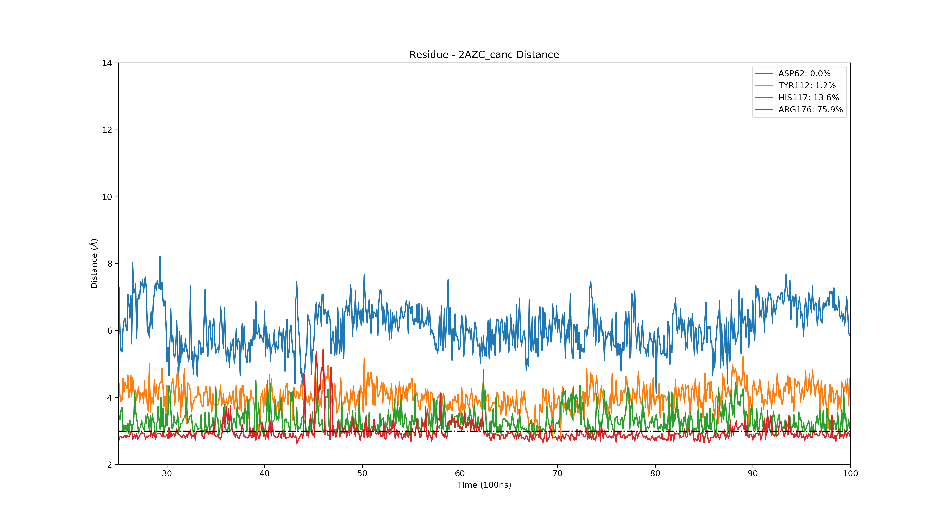
\includegraphics[width=.95\linewidth]{chapter4/2AZC_canc/2AZC_canc-dist_1.pdf}
  \end{subfigure}
  \\
  \begin{subfigure}{.45\textwidth}
     \centering
     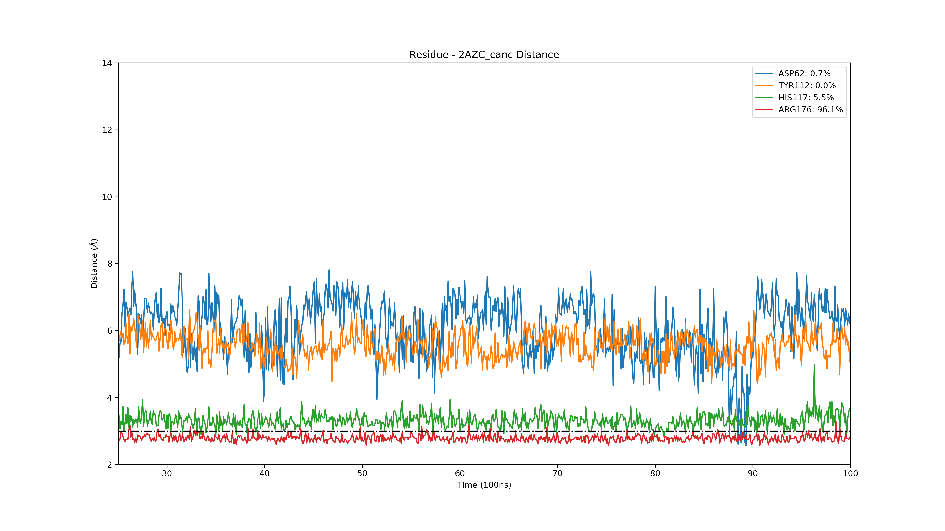
\includegraphics[width=.95\linewidth]{chapter4/2AZC_canc/2AZC_canc-dist_2.pdf}
  \end{subfigure}
    \begin{subfigure}{.45\textwidth}
     \centering
     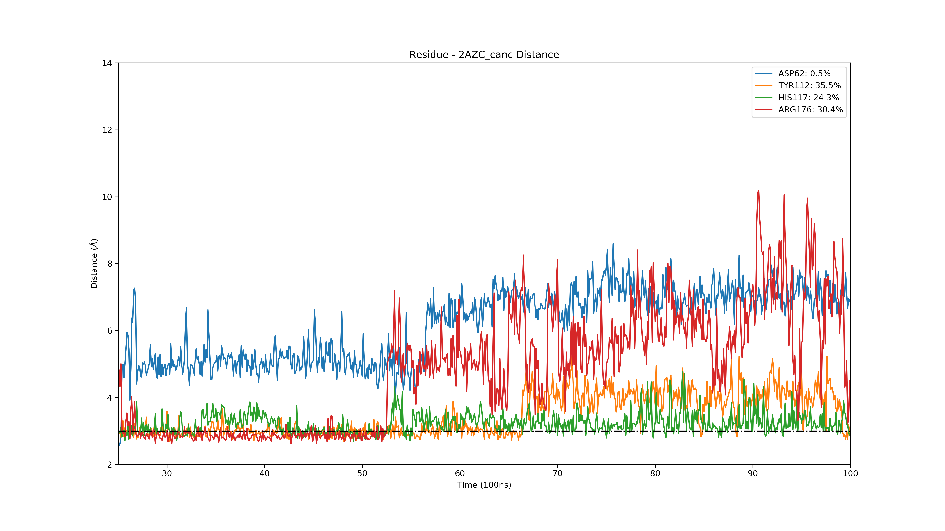
\includegraphics[width=.95\linewidth]{chapter4/2AZC_canc/2AZC_canc-dist_4.pdf}
  \end{subfigure}
\caption{Distance to key residues for 2AZC in the canonical binding mode from the other 4 MD simulations, not shown in Fig.\ref{fig:2AZC_canc-dist}. Each colored line represents the contact distance to a key residue.}
\label{sup:2AZC_canc-dist}
\end{figure}  


\begin{figure}[!ht]
\centering
  \begin{subfigure}{.45\textwidth}
     \centering
     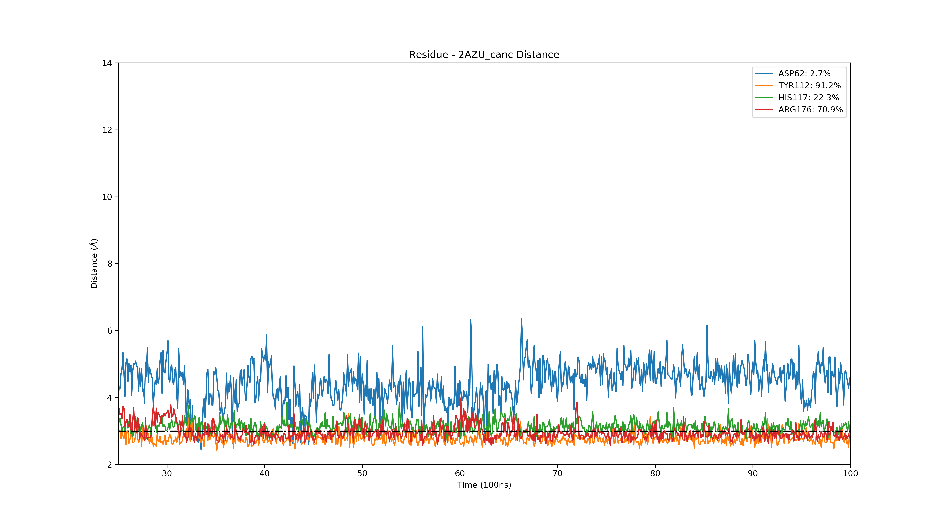
\includegraphics[width=.95\linewidth]{chapter4/2AZU_canc/2AZU_canc-dist_0.pdf}
  \end{subfigure}
  \begin{subfigure}{.45\textwidth}
     \centering
     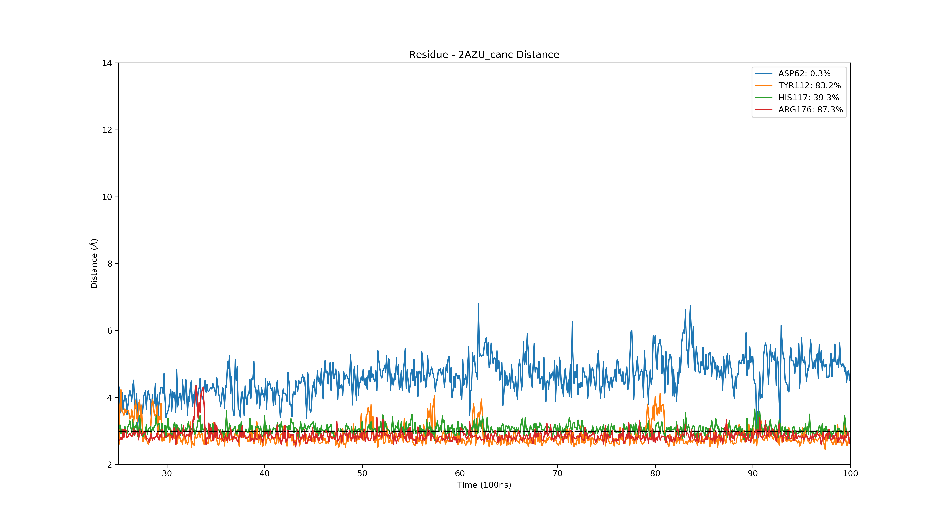
\includegraphics[width=.95\linewidth]{chapter4/2AZU_canc/2AZU_canc-dist_1.pdf}
  \end{subfigure}
  \\
  \begin{subfigure}{.45\textwidth}
     \centering
     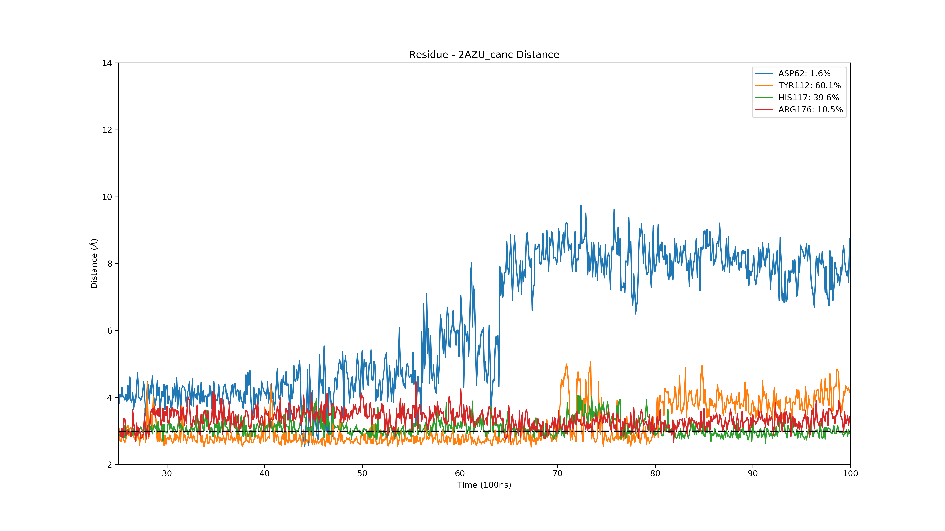
\includegraphics[width=.95\linewidth]{chapter4/2AZU_canc/2AZU_canc-dist_2.pdf}
  \end{subfigure}
    \begin{subfigure}{.45\textwidth}
     \centering
     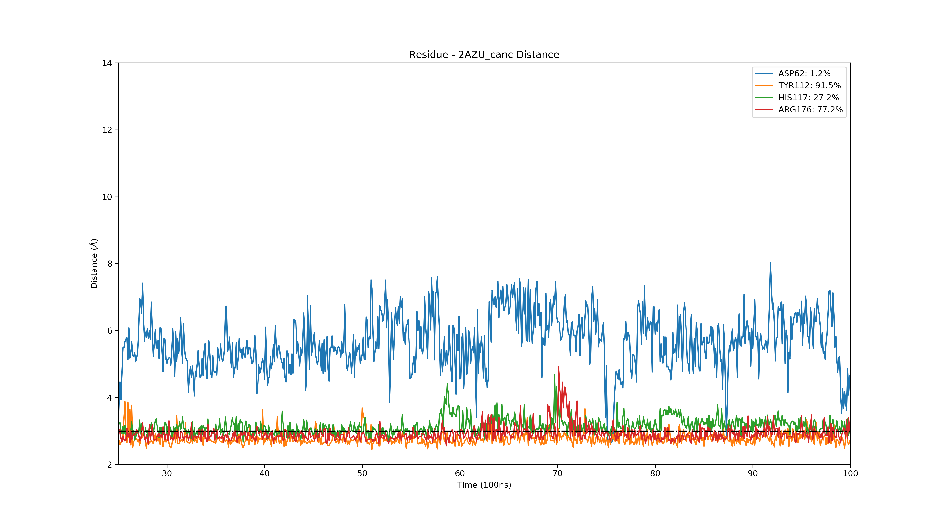
\includegraphics[width=.95\linewidth]{chapter4/2AZU_canc/2AZU_canc-dist_3.pdf}
  \end{subfigure}
\caption{Distance to key residues for 2AZU in the canonical binding mode from the other 4 MD simulations, not shown in Fig.\ref{fig:2AZU_canc-dist}. Each colored line represents the contact distance to a key residue.}
\label{sup:2AZU_canc-dist}
\end{figure}  

\begin{figure}[!ht]
\centering
  \begin{subfigure}{.45\textwidth}
     \centering
     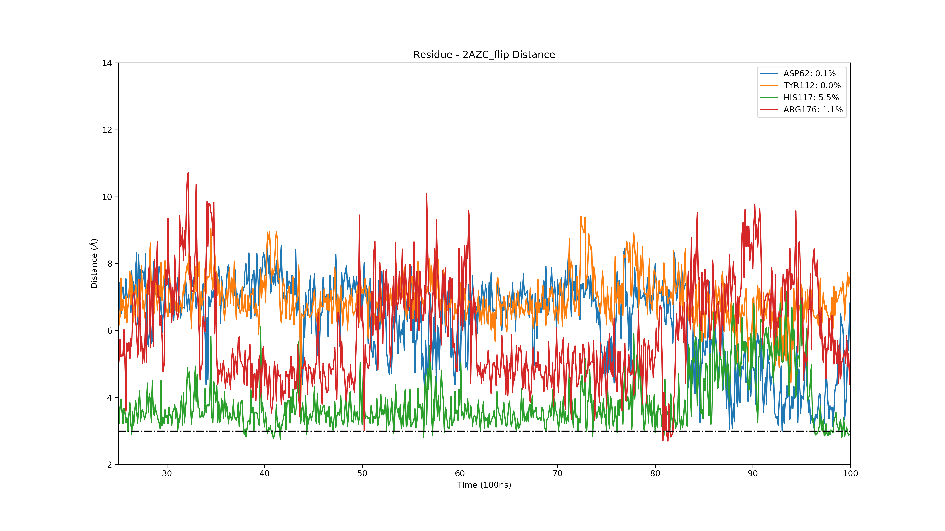
\includegraphics[width=.95\linewidth]{chapter4/2AZC_flip/2AZC_flip-dist_0.pdf}
  \end{subfigure}
  \begin{subfigure}{.45\textwidth}
     \centering
     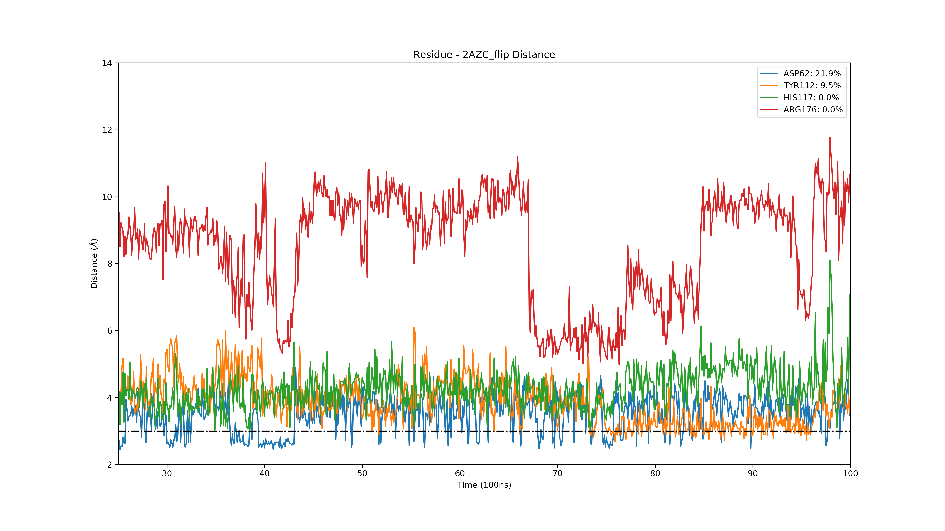
\includegraphics[width=.95\linewidth]{chapter4/2AZC_flip/2AZC_flip-dist_1.pdf}
  \end{subfigure}
  \\
  \begin{subfigure}{.45\textwidth}
     \centering
     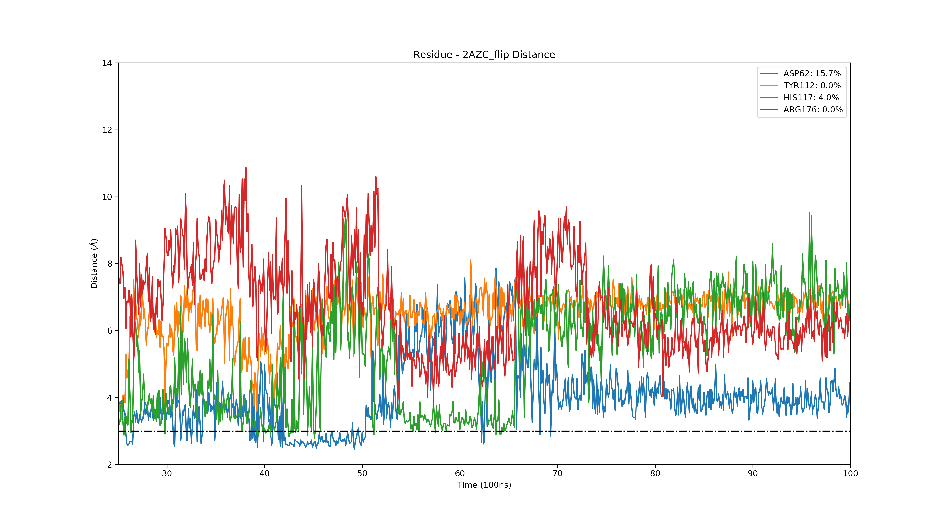
\includegraphics[width=.95\linewidth]{chapter4/2AZC_flip/2AZC_flip-dist_2.pdf}
  \end{subfigure}
    \begin{subfigure}{.45\textwidth}
     \centering
     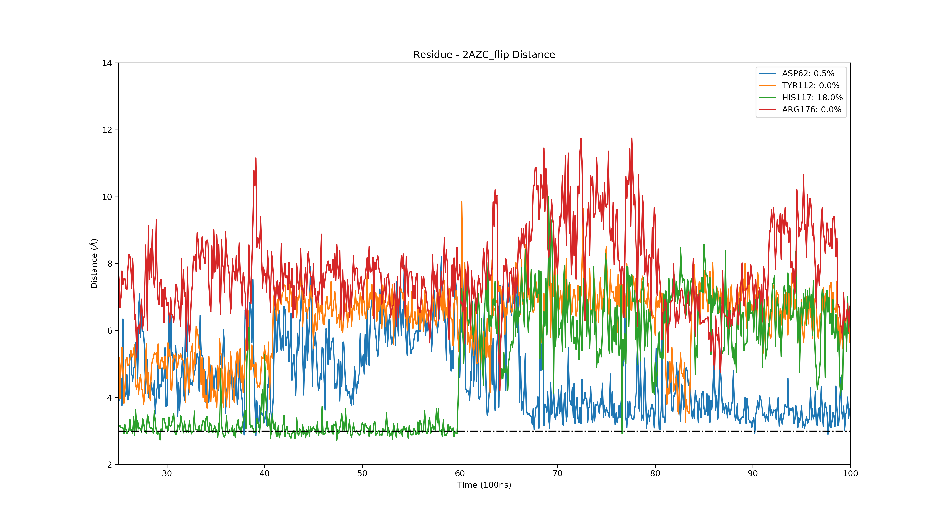
\includegraphics[width=.95\linewidth]{chapter4/2AZC_flip/2AZC_flip-dist_4.pdf}
  \end{subfigure}
\caption{Distance to key residues for 2AZC in the flipped binding mode from the other 4 MD simulations, not shown in Fig.\ref{fig:2AZC_flip-dist}. Each colored line represents the contact distance to a key residue.}
\label{sup:2AZC_flip-dist}
\end{figure}  

\begin{figure}[!ht]
\centering
  \begin{subfigure}{.45\textwidth}
     \centering
     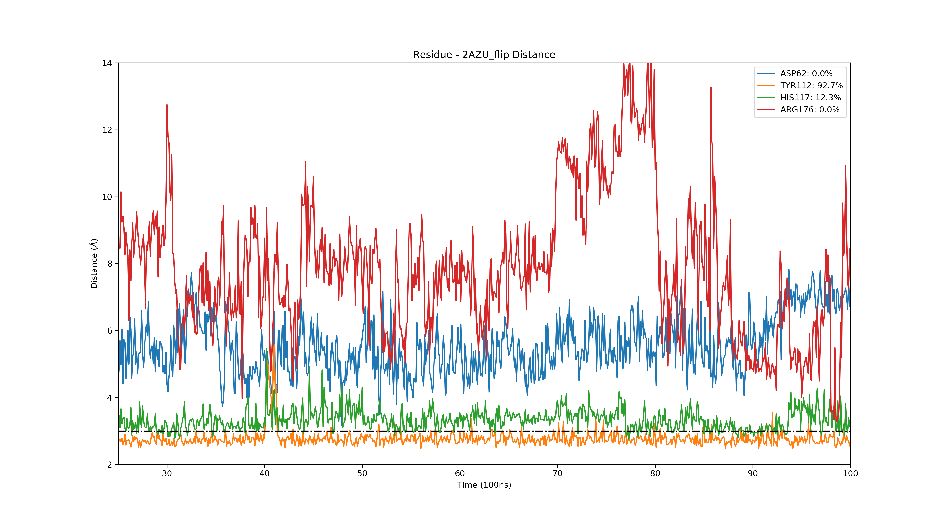
\includegraphics[width=.95\linewidth]{chapter4/2AZU_flip/2AZU_flip-dist_0.pdf}
  \end{subfigure}
  \begin{subfigure}{.45\textwidth}
     \centering
     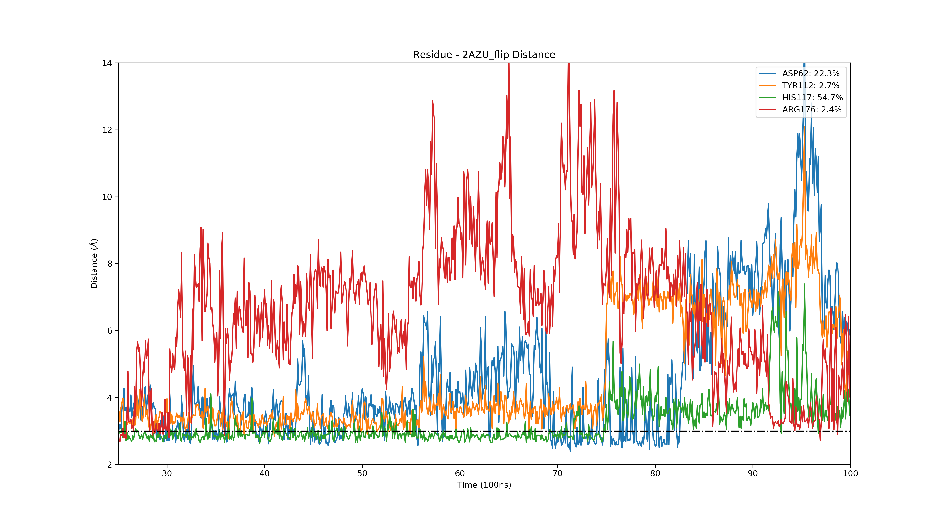
\includegraphics[width=.95\linewidth]{chapter4/2AZU_flip/2AZU_flip-dist_1.pdf}
  \end{subfigure}
  \\
  \begin{subfigure}{.45\textwidth}
     \centering
     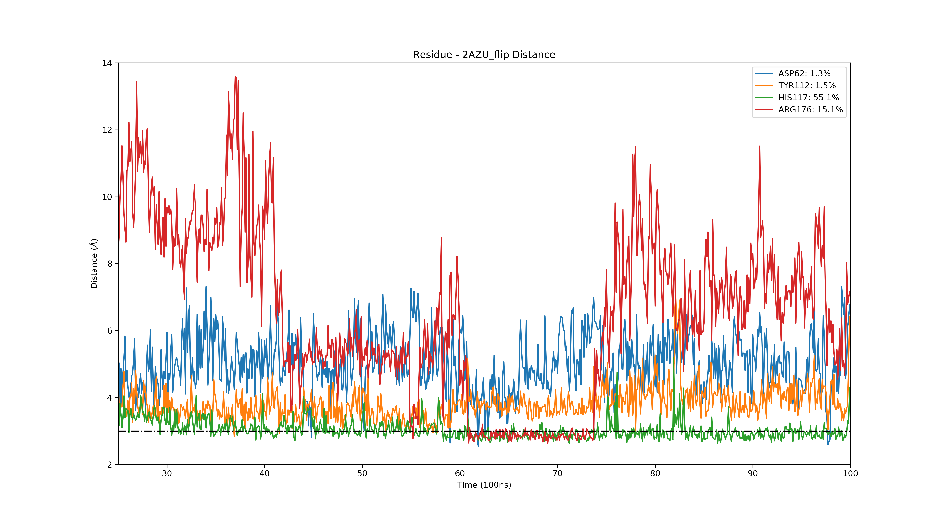
\includegraphics[width=.95\linewidth]{chapter4/2AZU_flip/2AZU_flip-dist_2.pdf}
  \end{subfigure}
    \begin{subfigure}{.45\textwidth}
     \centering
     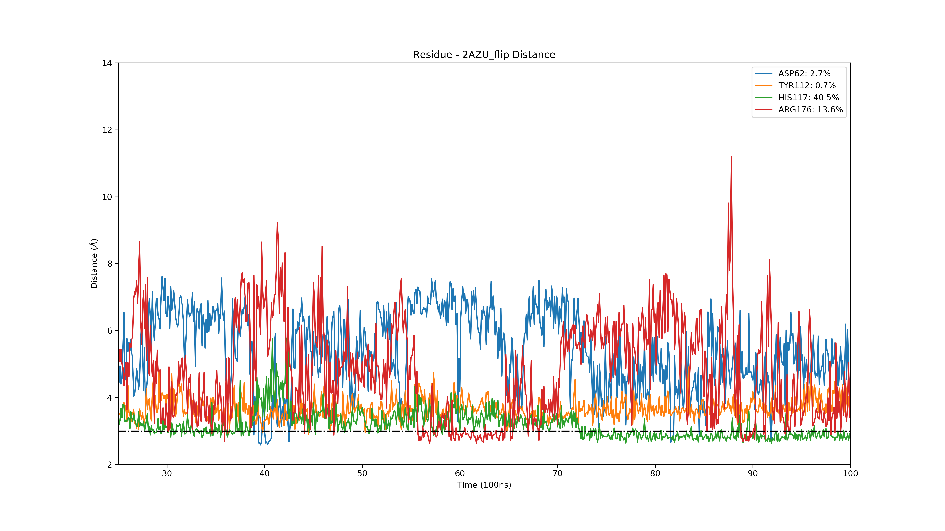
\includegraphics[width=.95\linewidth]{chapter4/2AZU_flip/2AZU_flip-dist_3.pdf}
  \end{subfigure}
\caption{Distance to key residues for 2AZU in the flipped binding mode from the other 4 MD simulations, not shown in Fig.\ref{fig:2AZU_flip-dist}. Each colored line represents the contact distance to a key residue.}
\label{sup:2AZU_flip-dist}
\end{figure}  